%%%%%%%% ICML 2020 EXAMPLE LATEX SUBMISSION FILE %%%%%%%%%%%%%%%%%

\documentclass{article}

% Recommended, but optional, packages for figures and better typesetting:
\usepackage{microtype}
\usepackage{graphicx}
\usepackage{subfigure}
\usepackage{booktabs} % for professional tables
\usepackage{amssymb}


% hyperref makes hyperlinks in the resulting PDF.
% If your build breaks (sometimes temporarily if a hyperlink spans a page)
% please comment out the following usepackage line and replace
% \usepackage{icml2020} with \usepackage[nohyperref]{icml2020} above.
\usepackage{hyperref}
\usepackage{cleveref}
\usepackage{pdfpages}

% Attempt to make hyperref and algorithmic work together better:
\newcommand{\theHalgorithm}{\arabic{algorithm}}

% Use the following line for the initial blind version submitted for review:
\usepackage[accepted]{icml2020}

% If accepted, instead use the following line for the camera-ready submission:
%\usepackage[accepted]{icml2020}

% The \icmltitle you define below is probably too long as a header.
% Therefore, a short form for the running title is supplied here:
\icmltitlerunning{Multi-scale learning on graphs}

\begin{document}

\twocolumn[
\icmltitle{Multi-Scale Learning on Graphs}

% It is OKAY to include author information, even for blind
% submissions: the style file will automatically remove it for you
% unless you've provided the [accepted] option to the icml2020
% package.

% List of affiliations: The first argument should be a (short)
% identifier you will use later to specify author affiliations
% Academic affiliations should list Department, University, City, Region, Country
% Industry affiliations should list Company, City, Region, Country

% You can specify symbols, otherwise they are numbered in order.
% Ideally, you should not use this facility. Affiliations will be numbered
% in order of appearance and this is the preferred way.
\icmlsetsymbol{equal}{*}

\begin{icmlauthorlist}
%\icmlauthor{Aeiau Zzzz}{equal,to}
%\icmlauthor{Bauiu C.~Yyyy}{equal,to,goo}
%\icmlauthor{Cieua Vvvvv}{goo}
%\icmlauthor{Iaesut Saoeu}{ed}
%\icmlauthor{Fiuea Rrrr}{to}
%\icmlauthor{Tateu H.~Yasehe}{ed,to,goo}
%\icmlauthor{Aaoeu Iasoh}{goo}
%\icmlauthor{Buiui Eueu}{ed}
%\icmlauthor{Aeuia Zzzz}{ed}
%\icmlauthor{Bieea C.~Yyyy}{to,goo}
%\icmlauthor{Teoau Xxxx}{ed}
\icmlauthor{Franz Rieger}{tum}
\end{icmlauthorlist}

\icmlaffiliation{tum}{Department of Informatics, Technical University of Munich, Munich, Germany}
%\icmlaffiliation{goo}{Googol ShallowMind, New London, Michigan, USA}
%\icmlaffiliation{ed}{School of Computation, University of Edenborrow, Edenborrow, United Kingdom}

\icmlcorrespondingauthor{Franz Rieger}{riegerfr@cs.tum.edu}
%\icmlcorrespondingauthor{Eee Pppp}{ep@eden.co.uk}

% You may provide any keywords that you
% find helpful for describing your paper; these are used to populate
% the "keywords" metadata in the PDF but will not be shown in the document
\icmlkeywords{Machine Learning, ICML}

\vskip 0.3in
]

% this must go after the closing bracket ] following \twocolumn[ ...

% This command actually creates the footnote in the first column
% listing the affiliations and the copyright notice.
% The command takes one argument, which is text to display at the start of the footnote.
% The \icmlEqualContribution command is standard text for equal contribution.
% Remove it (just {}) if you do not need this facility.

\printAffiliationsAndNotice{}  % leave blank if no need to mention equal contribution
%\printAffiliationsAndNotice % otherwise use the standard text.

\begin{abstract}
This seminar paper discusses several approaches for multi-scale learning on graphs, their use-cases and trade-offs. % It presents methods based on spatial and spectral convolutions. 
 Spectral methods like wavelets and scattering transforms can be applied without the need to train and are flexible w.r.t.\ scale. % and rely on convolutions in the spectral domain. 
 Spatial methods operating on different scales like graph coarsening, hierarchical clustering or graph neural network (GNN) architectures rely on spatial convolutions in the vertex domain. Some modern methods combine spectral with spatial approaches for better performance. % for graph coarsening, hierarchical clustering or architectures operating on multiple scales.
\end{abstract}

\section{Introduction}
\label{introduction}
Recently, learning on graphs has become an important and active subject of study. It can be applied to a variety of problem statements, such as predicting the spread of a novel disease over a population \cite{hammond2011wavelets}, as well as problems on other real-world graphs like citation networks, brain connectomes, social networks or molecules. In fact, modern GNN approaches as well as classical spectral methods on graphs have made tremendous progress in tackling challenging tasks like semi-supervised node classification, graph classification, link prediction, community detection and the generation of node embeddings. This is reflected in the abundance of survey papers discussing this topic \cite{ zhang2020deep, zhou2018graph, wu2020comprehensive, ortega2018graph, bronstein2017geometric}.

 In this paper we discuss multi-scale learning on graphs. 
 On the one hand, multi-scale can be viewed as the number of nodes in different graphs. Therefore, we review methods %for smaller and larger graphs, as well as methods
 which are flexible in the size of the graphs they are dealing with. On the other hand, methods need to operate on different scales when processing a single graph: On the small scale, one can observe a node together with its immediate neighbors. Correspondingly, at bigger scales, further away nodes are relevant. Consequently, at the global scale, the whole graph is observed. Therefore, different kinds of information are processed at different scales. This can be seen intuitively as different levels of abstraction, e.g.\ in a graph modeling a population different scales refer to individuals, households or cities respectively. This view will prove helpful when discussing hierarchical clustering.
 An undirected graph can be represented by its $N$ nodes with node features $\mathbf{X}\in \mathbb{R}^{N\times m}$. %$\mathcal{V}$.
 Its (weighted) edges between the nodes are defined through its symmetric non-negative adjacency matrix $\mathbf{A}\in \mathbb{R}_+^{N\times N}$, where $\mathbf{A}_{i,j}$ corresponds to the weight of the edge between the nodes $i$ and $j$. Real-world graphs are oftentimes sparse, i.e.\ the number of edges depends linearly on $N$, which is relevant for computational complexity.


%spectral: decompose signal into frequency/wavelets...
%laplacian: diffuse potential/heat given to node

Most of the approaches presented here implicitly rely on the homophily assumption, which states that neighboring nodes are more similar to each other than nodes which are further apart. Oftentimes, these methods on graphs are analogous to existing approaches on euclidean data like images.
This especially holds for convolutions \cite{he2016deep} whose definition on graphs is not as straightforward as convolutions on image data, where the pixels follow a clear grid structure.
As we will see, on graphs we distinguish between spatial and spectral convolutions \cite{bruna2014spectral}: 
\textbf{Spatial convolutions} are localized in the vertex domain, where a node in a graph is influenced by its neighbors, much like a pixel's value in an image depends on its surrounding pixels. However, the neighbors cannot be ordered like pixels nor is their count fixed. Therefore, most GNNs perform some form of (repeated) message passing, where the node embeddings of the neighbors are aggregated for each node and then some computation is performed to update the embeddings. Methods working in the spatial domain are discussed in \Cref{sec:SpatialMethods}. 
% (TODO: Introduce GNNs properly, explain problem: oversmoothing)
%A common GNN architecture is the Graph Convolutional Network \cite{kipf2016semi}, where one layer updating the node's representation can be described as 
%Most GNN architectures update the representation of node $i$ in one layer as follows:\\
%$ \mathbf{X}^{(n+1)}_i = \textrm{F}(\mathbf{X}^{(n)}_i, \textrm{mean}_{j \in \mathcal{N}(i)}( \textrm{G} ( \mathbf{X}^{(n)}_i, \mathbf{X}^{(n)}_j, \mathbf{A}_{i,j})) )$ Here, F and G can be trainable functions like MLPs, $\mathcal{N}$ refers to the neighbors and mean can be replaced by any permutation invariant function like a max operator \cite{wu2020comprehensive}.
 \textbf{Spectral convolutions} however are localized in the graph's frequency domain as we will see in the next section. They rely on the convolution theorem%\footnote{\href{https://en.wikipedia.org/wiki/Convolution_theorem}{https://en.wikipedia.org/wiki/Convolution\_theorem}}
 , which states that a multiplication in the frequency domain corresponds to a convolution in the spatial domain (see \Cref{sec:convtheorem}).

%fourier transformation:\footnote{\href{https://en.wikipedia.org/wiki/Fourier\_transform}{https://en.wikipedia.org/wiki/Fourier\_transform}}


%\cite{hammond2011wavelets}  In the following, we present different approaches for learning on graphs on multiple scales, ranging from spectral methods like wavelets and graph scattering transforms to Graph Neural Network based architectures.

% and most GNNs use this app



%A symmetric, connected graph $G = (V,E, w, g)$, consists of $N=|V|$ vertices, $m = |E|$ (possibly directed) edges $ E \subseteq V^2$. The edges are weighted $ w: V^2 \to \mathbb{R}$ and the vertices receive features $ g: V\to \mathbb{R}^m $. Based on the weights, we can define an adjacency matrix: $A_{u,v} = w(u,v) = w_{u,v}$ for $u,v \in V$. For spectral methods, we define the weighted degree matrix $D = ???$ and the Laplacian $L = D-A$ of a graph. For a connected graph, its eigenvalues (also frequencies of the graph) and eigenvectors ($L\mathbf{\chi}_i = \lambda_i \mathbf{\chi}_i$) exist because the Laplacian is symmetric(?) and can be ordered w.l.o.g. such that $0 = \lambda_0 < \lambda_1 \leq \lambda_2 \leq \ldots \leq \lambda_i \leq \ldots \leq \lambda_{N-1}$. (notation from: \cite{hammond2011wavelets} )

%Analogously to Fourier transformations on classical data (see appendix?), we can also define a Fourier transformation on graphs, where instead of mapping a continuous function to the frequency domain, we map a function $f \in \mathbb{R}^N$ which assigns a value to each vertex in the graph to a function which assigns a value to each eigenvalues (and corresponding eigenvector) of the Laplacian, where low eigenvalues correspond to low frequencies (i.e. the feature does not change much throughout the graph), whereas high eigenvalues correspond to a high frequency change from a node to its neighbors.
%Mathematically, the graph Fourier transform is defined by $\hat{f}(l) = \langle \mathbf{\chi}_l, f\rangle = \sum_{n = 1}^{N}\mathbf{\chi}_l(n)f(n)$. Its inverse follows as $f(n) = \sum_{l = 0}^{N-1}\hat{f}(l) \mathbf{\chi}_l(n)$.








\section{Spectral Methods}
\label{SpectralMethods}

Spectral methods are very useful approaches which oftentimes do not even require any training to work. Similar to Fourier Transformation on Euclidean data\footnote{\href{https://en.wikipedia.org/wiki/Fourier\_transform}{https://en.wikipedia.org/wiki/Fourier\_transform}}, Graph Fourier Transformation is applied to transform a graph to the spectral frequency domain.
%To define the spectral frequency domain of a graph for spectral convolution, Graph Fourier Transformation is applied similarly to Fourier Transformation on euclidean data:
We first define the degree matrix of a graph as $\mathbf{D}=\textrm{diag}(\sum_{i =1}^{N} \mathbf{A}_{1,i}, \ldots, \sum_{i =1}^{N} \mathbf{A}_{N,i})$ and the Laplacian matrix as $\mathbf{L} =\mathbf{D}-\mathbf{A}$. Then, the eigenvalues and eigenvectors ($\mathbf{L} \mathbf{\chi}_l = \lambda_l \mathbf{\chi}_l$) of the Laplacian are of central importance for spectral methods. The eigenvalues $\lambda_l$ can be seen as the discrete frequencies of a graph, where the corresponding eigenvector $\mathbf{\chi}_l$ assigns an amplitude to each node in the graph. A low eigenvalue corresponds to a low frequency, which means that nearby nodes get assigned similar values by the corresponding eigenvector. % and the values only change slowly throughout the graph.
 Accordingly, high eigenvalues correspond to higher frequencies (noise) and the values assigned by the corresponding eigenvector change faster for adjacent nodes. %(Therefore, if we just use the first few eigenvectors with the lowest eigenvalues, we can roughly reconstruct the graph.)
 Spectral clustering methods \cite{ng2002spectral} use this property to obtain node embeddings from the corresponding entries in the eigenvectors.
Now we can define the graph Fourier transform of a signal on nodes (e.g.\ the node features $\mathbf{X}$) $f:[N] \to \mathbb{R}^m$ to a signal on eigenvectors $\hat{f}(l) =\sum_{i = 1}^{N}\mathbf{\chi}_l(i)f(i)$. We can restore the signal to the spatial domain through the inverse which follows as $f(i) = \sum_{l = 0}^{N-1}\hat{f}(l) \mathbf{\chi}_l(i)$. 


%\subsection{Wavelets}
\textbf{Wavelets} % \label{wavelets}
Spectral graph wavelets, as introduced by \citet{hammond2011wavelets} can be represented by a quadratic matrix $\mathbf{\Psi}$. Here, $\mathbf{\Psi}_{i,j}$ denotes how relevant the embedding of node $i$ is for the calculation of the new embedding of node $j$, which aggregates over all nodes $i$ according to the relevance.
This gives a notion for (unlearned) convolution on graphs in the vertex domain, as an alternative to simply just considering the neighbors of a node as GNNs do.
With the graph Fourier transform, we can now apply the convolution theorem to define global convolutions in the frequency domain on graphs \cite{bruna2014spectral}: A wavelet kernel $g(t\lambda)$ of scale $t>0$ (which is not to be confused with the corresponding graph wavelet $\mathbf{\Psi}^t$), assigns relevance to different frequencies (eigenvalues).
%Wavelets can be used to empathize on different frequencies: For wavelets, a (parameterized?) kernel function $g: \mathbb{R} \to \mathbb{R}^+$ 
It is utilized to define a spectral graph wavelet transform operator $\widehat{T_gf}(l) = g(\lambda_l)\hat{f}(l)$ by multiplying the signal in the frequency domain.
The inverse follows as $(T_gf)(i) = \sum_{l=0}^{N-1}g(\lambda_l)\hat{f}(l)\mathbf{\chi}_l(i)$. Note that the explicit wavelet $\mathbf{\Psi}^t_{i,j} = \sum_{l=0}^{N-1} g(t\lambda_l)\mathbf{\chi}_l(i)\mathbf{\chi}_l(j)$ does not depend on the signal on the graph. With this definition of wavelets, using a hand-selected or learned kernel function $g: \mathbb{R^+}\to \mathbb{R}$ (which converges to $0$ for increasing eigenvalues) and a set of different scales $t_1, \ldots, t_k >0$ we can now convolve any signal using $k$ different wavelets (of local to global scale) as shown in \Cref{fig:wavelets}.  Different wavelet kernels and scales can also be combined in a filter-bank of wavelets. Since the wavelets are usually sparse, this method works faster than graph Fourier Transform with dense eigenvectors.

\begin{figure}%[ht]
	%\vskip 0.2in
	\begin{center}
		\centerline{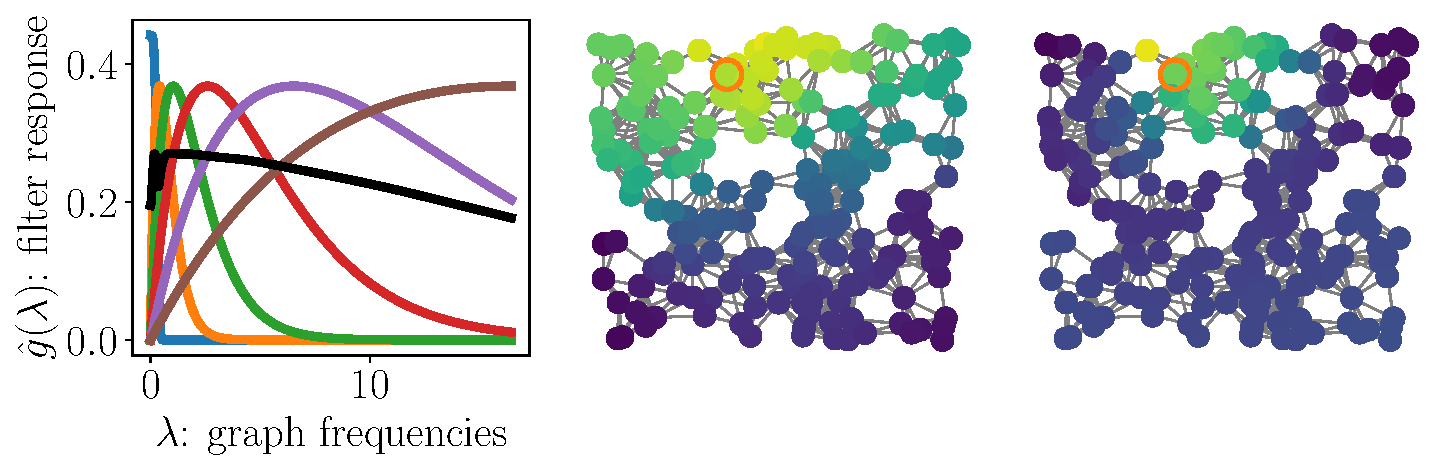
\includegraphics[width=\columnwidth]{wavelets}}
		%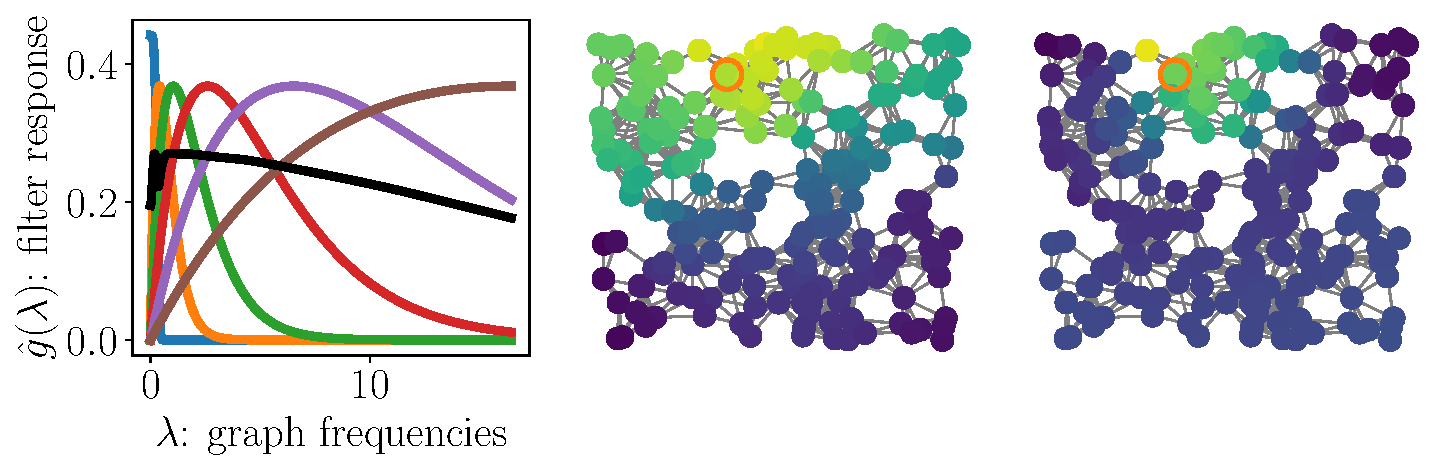
\includepdf[width=\columnwidth]{wavelets.pdf}
		%\include{wavelets.pgf}
		\vskip -0.1in
		\caption{
			%Wavelets on different scales as kernels on a sensor graph using PyGSP\footnote{ \href{https://pygsp.readthedocs.io}{https://pygsp.readthedocs.io}}. 
			(left) Filterbank of wavelets: sensitivity w.r.t.\ the graph frequencies $\lambda$. (middle and right) Wavelets of different scales localized around the same circled node. Brighter colors correspond to higher relevance for that node. Note how the nodes in the top left corner, a nearby cluster to the selected node, receive high importance for one scale (low frequency), but a lower importance for the other scale (higher frequency). Created with \href{https://pygsp.readthedocs.io}{PyGSP}. %\footnotemark.%\footnote{ }.
		}
		\label{fig:wavelets}
	\end{center}
	\vskip -0.4in
\end{figure}

%\footnotetext{\href{https://pygsp.readthedocs.io}{https://pygsp.readthedocs.io}}

%There are many ways to define wavelets, when working on the spectrum, we can use a graph wavelet kernel $g(t\lambda): \mathbb{R}\to \mathbb{R}$ which can operate on different scales $t$.
%With this operator, the graph wavelets follow as 


As discussed by \citet{Shuman_2013} spectral graph wavelet transform is not the only way to define wavelets. For example, \citet{crovella2003graph} define wavelets based on a wavelet kernel function on the number of hops between a node and the node around which the wavelet is centralized. Other popular wavelets follow different intuitions: Diffusion wavelets \cite{coifman2006diffusion} analyze the spread of heat through the graph over different timescales, starting at the node they are localized around% (can also be estimated with spectral methods \cite{todo})
. For tree-based wavelets \cite{ram2011generalized} a tree is constructed by grouping together similar datapoints. Average interpolating wavelets \cite{rustamov2011average} are created by interpolating between nodes.
%\cite{narang2012multi} (not important)
Some architectures combine wavelets with learning tasks by making the wavelets learnable \cite{gavish2010multiscale}.
Similar to previous work \cite{bruna2014spectral, henaff2015deep}, \citet{defferrard2016convolutional} pick up this idea and instead of using a constant wavelet kernel, $g$ is a polynomial on $\lambda$ with trainable coefficients, which are independent on the graph size. Correspondingly, CayleyNets \cite{levie2018cayleynets} efficiently use Cayley polynomials for the kernel, which allows learning spectral filters that specialize in the important frequencies or scales. %With that, the convolutions are again localized on the nodes and the architecture scales linearly with the number of edges.

More modern architectures like Graph Wavelet Neural Network (GWNN) \cite{ xu2019graph} combine spectral wavelets into a GNN for node classification in a sparse, efficient manner, where the convolution is localized in vertex domain. This method is more flexible w.r.t.\ the neighborhood of a node compared to the previously mentioned node hop wavelets \cite{crovella2003graph}.
% convolution,flexible neighborhood, faster than Fourier since graph wavelets are typically sparse in comparison to dense eigenvectors of the Laplacian.
To compute node embeddings with wavelets, \citet{donnat2018learning} use heat diffusion wavelets, where the distribution of the nodes' wavelet coefficients is compared to assign similar embeddings to similar distributions.
%4\cite{bruna2013spectral}: defines convolution architectures on graphs (spatial/ especially spectral, show analogously to images (subsampling pixels))
%\cite{defferrard2016convolutional} : builds on previous: spectral cnn, works locally (nice formulation of $\hat{x} = U^Tx$, $x =U\hat{x} $), $L = UVU^T$
%\cite{ henaff2015deep} multiple input channels, learn weights $x*_Gg = U^T(diag(w_g)Ux)$
%Spectral filters can capture global structure (can be localized with smoothing in the spectral domain \cite{bruna2013spectral}) (other than local methods like (shallow) GCN \cite{kipf2016semi})
 As computing the full eigendecomposition of the Laplacian is computationally expensive, many methods just compute the first few lowest eigenvectors. % (i.e. through power iteration) 
 With the homophily assumption, this approximation is justified because they already convey most of the low noise information, which is needed to reconstruct the rough structure of the graph%(assuming homophily again)
. In contrast to that, Lanczosnet \cite{liao2019lanczosnet} computes a low rank approximation of the Laplacian %(whose potentiation is then cheap) 
using the Lanczos algorithm to efficiently use information from higher frequencies. Which frequencies the model focuses on can again be learned. %.  multiple scales (of eigenvalues and therefore frequencies) and therefore enables learning spectral filters and which frequencies are most relevant.
 In contrast to most wavelets, which only depend on the topology of the graph, \citet{rustamov2013wavelets} also consider the class of signals, which will be defined on the graph, to construct wavelets which can sparsely represent these signals.




%\subsection{Graph Scattering Transforms}
\textbf{Scattering Transforms}
%\label{GraphScatteringTransforms}
Graph Scattering Transforms, as defined by \citet{zou2019graph}, are an extension of scattering transforms in euclidean space \cite{bruna2013invariant}. As a spectral method, they rely on a filter bank of graph wavelets as convolutional filters, which are applied in multiple layers to form a powerful feature extractor. They transform a signal on a graph by repeatedly applying the wavelet operator, possibly for different scales, to the graph as illustrated in Appendix \Cref{fig:scatteringresult}. Then, the embeddings of all the layers can be concatenated for further processing. % and averaged concatenate all the layers, where an averaging operator is applied to each layer.
%By transforming images into graphs of pixels which are connected to their surrounding pixels, graph scattering transforms can be applied to the pixels' values as illustrated in appendix \Cref{fig:scatteringresult}. 
After reducing the dimensionality of the output and applying a simple MLP, the signal can be used for classification or community detection in graphs. This shows that graph scattering transforms are able to extract important information without training, which is very powerful when little to no training data is available. %(still depend on selection of wavelet scale)
 %For illustration of the image classification refer to \cref{fig:scatteringresult} (Appendix)
A similar scattering transform method is described by \citet{gao2019geometric}, where the normalized moments of the data are used.

\citet{gama2019diffusion} show that diffusion graph scattering transforms are also stable w.r.t.\ perturbations in the metric domain while still being able to capture high frequency information.
Furthermore they are robust to graph manipulations like deformations. 
\citet{gama2019stability} also extend graph scattering transforms to multiresolution wavelets, allowing for 'learning' on multiple scales without loosing its robustness property. Alternatively, \citet{chen2014unsupervised} use haar wavelets for scattering transforms and an unsupervised learning algorithm, which can also perform well on unknown graph topologies, operate on different scales and are again robust to permutations.
While the wavelets of Graph Scattering Transforms are usually selected manually and not learned, one possible extension to graph scattering transforms would be also training the wavelet kernels like in CayleyNets.

\section{Spatial Methods}
\label{sec:SpatialMethods}

In contrast to the spectral methods we saw so far, we now present several approaches for multi-scale learning on graphs, which employ GNNs with spatial convolutions in the vertex domain. These approaches are oftentimes computationally cheaper and perform better than spectral methods.
%modern approaches for multi-scale learning on graphs, most of which are based on GNNs.
 We include methods for coarsening graphs before further processing, hierarchical clustering, as well as a view on different GNN architectures and how they deal with different scales. For a short discussion of methods specialized on specific graphs and sizes refer to \Cref{sec:other}.



%\subsection{Scaleable GNN architectures}
\textbf{Multi-scale GNN architectures}
Classical GNNs usually aggregate the node embeddings of the direct neighbors. While multiple layers can be stacked, so that also information from multiple hops can reach a node, their performance degrades with increasing depth, which limits the scale of this approach. To address this issue called oversmoothing and to improve performance on larger scales, Multi-hop Hierarchical Graph Neural Networks %(MHGNNs)
\cite{xue2020multi} concatenate the features obtained from multiple message-passing hops. %, where the features for all the nodes in the same hop-level are aggregated into a single embedding. 
To aggregate the embeddings for all the nodes, attention mechanisms (like proved useful in other domains like Machine Translation \cite{vaswani2017attention}) are employed to direct importance to the most relevant nodes in the hops.
Similarly, the architecture of \citet{abuelhaija2019mixhop} also aggregates node embeddings from multiple hops by computing powers of the adjacency matrix in a fast manner. Another approach for using GNNs for learning on a larger scale are residual connections to address the vanishing gradient problem, which occurs when stacking many layers \cite{li2019deepgcns}.

Instead of using several layers to reach further away information, the approach presented by  \citet{klicpera_predict_2019} first approximates a personalized PageRank score for every node, which assigns relevance for the other nodes.  
Then it computes new node embeddings for each node and aggregates them utilizing the PageRank score. Even though this approach allows for infinite depth, the performance does not degrade as the score is localized for every node. The scale of this assignment can be adjusted similar to wavelets by changing the restart probability \cite{page1999pagerank}.
 Alternatively, Graph diffusion convolution (GDC) \cite{ klicpera2019diffusion} can be utilized: It combines spectral approaches with GNNs by transforming the input graph, using diffusion to define the weights of the edges, which are then sparsified. Afterwards any GNN method can be applied on the new graph. Similarly, adaptive graph convolutions \cite{li2018adaptive} learn a residual Laplacian for each graph, which increases local consistency and lets the architecture deal well with different graph sizes.
Yet one more notable approach is introduced in \citet{abu2018n}, where first new edges are discovered by random walks of different lengths, covering different scales. Then, training is performed on the new edges with a combination of different GNNs.


%\subsection{Graph Coarsening}
\textbf{Graph Coarsening} 
Since learning on large graphs is computationally expensive and the problem of oversmoothing appears, some methods first coarsen the graph by removing unimportant nodes while retaining relevant information, such that the graph becomes smaller and learning on multiple scales gets easier.
One very recent method using coarsening is GraphZoom \cite{deng2020graphzoom}, which combines several steps to generate node embeddings in an efficient, scalable manner: At first, it performs graph fusion to combine the original adjacency matrix and the node features into a single adjacency matrix. For that, another adjacency matrix is created by using similarity scores of the nodes' embeddings. This new matrix is then combined linearly with the original adjacency matrix to generate the fused graph without node features. To reduce computational complexity, the fused graph is then coarsened by repeatedly merging nodes with high similarity in their spectral embeddings, retaining relevant information (like by \citet{Shuman_2013}). With the coarsened graph, any node embedding method (spectral or GNN based) can be employed to generate useful node embeddings for the coarsened nodes of the top level. Then, the embeddings are projected back to the original, bottom level nodes by splitting the coarsened graph's nodes up in the same way they were merged in the coarsening step before. Afterwards, the embeddings are refined using a spectral low pass filter for smoothing.% The quality of the resulting embeddings is high as shown by the performance of the node classification and link-prediction tasks.

In comparison to existing methods like MILE \cite{liang2018mile} which also first coarsen a graph, compute coarse embeddings and then refine them to the original nodes, GraphZoom's refinement is not learned by a GNN model but performed by simple matrix multiplications. This saves training time and also increases performance for some tasks.
One possible improvement for GraphZoom could be found in the fusion step: The similarity matrix of the node embeddings is based on a coarsened graph to avoid the quadratic time complexity for the k-nearest-neighbor computation it uses. As a reviewer of the paper noted, existing methods like locality sensitive hashing (LSH) \cite{wang2014hashing} could improve the quality of the fused adjacency matrix and therefore also the overall performance. Since LSH does not take the topology of the graph into account, random walks \cite{ zhuang2018dual} would be another viable alternative for generating the similarity matrix.



%\subsection{Hierarchical clustering}
\textbf{Hierarchical clustering}
One other way of learning on multiple scales on graphs is hierarchical clustering, which might be viewed as several layers of graph coarsening.
The nodes of a graph are assigned to local clusters, which are then repeatedly assigned to (super-)clusters of clusters, which form a hierarchy. In this way, at lower levels close to the original graph, local information can be processed while on higher levels, global information can be passed through the superclusters.
As a prominent example, we discuss the Differential Pooling (DiffPool) architecture \cite{ying2018hierarchical}, which has proved especially helpful in graph classification. %, when a multi layer perceptron is applied after the last layer.
Internally, DiffPool consists of several layers, which subsequently pool the graph into smaller graphs. Each layer applies an assignment GNN to compute a soft assignment of each node to clusters and an embedding GNN to alter the embeddings. The clusters then build the nodes of the next layer by pooling together the edges and the new embeddings.

%Each layer takes an input a graph with its node embeddings and the adjacency matrix. In the layer, two distinct GNN models %(e.g.\ SAGEConv) 
%are applied to it: The embedding model computes the new embeddings for the nodes of the current layer. Meanwhile, the separate assignment model computes a soft assignment for each node of the current layer to clusters, which will become the nodes of the next layer. According to this soft assignment, the new node embeddings and the edges are then pooled to form the clusters of the next layer.
%In this way, the initial layers take into account for the low level features of a graph through the GCN layers which use the close neighbor's information, while the last layers allow the model to incorporate top-level information from the whole graph, therefore making use of different scales by building a hierarchical clustering.

One advantage of DiffPool is its flexibility w.r.t.\ the GNN models. Depending on the use case, simple GNNs (like SAGEConvs \cite{hamilton2017inductive}) but also advanced methods like GraphZoom for the updated embeddings or a spectral clustering method for the assignments can be applied.
With the soft assignment, DiffPool can flexibly learn the cluster assignments in a fully differentiable manner, which allows it to determine the appropriate number of clusters to use. This is an improvement to other methods that depend on a spectral clustering subroutine, which produces a fixed (and therefore possibly sub-optimal) number of clusters \cite{defferrard2016convolutional}. 
However, the maximal number of clusters in each layer after the initial graph still needs to be defined beforehand, posing difficulties when dealing with a dataset which contains graphs with a high variance in the number of nodes. This could be alleviated by flexibly defining the maximal number of nodes as a ratio of the input nodes of the specific graph. Then, the assignment model is conditioned on multiple random but constant values for each cluster and a softmax function is applied to the assignment scores. % instead of assigning them to the same (number of predefined) clusters for all graphs. %(much like spectral random ...\cite{todo})
Another drawback of DiffPool is its quadratic space complexity in the number of clusters: due to the soft assignment, the pooled graphs are usually fully connected and not sparse anymore.% This means that the number of edges is quadratic in the number of clusters. %, which is especially relevant for the first layer since it has the most clusters.

Therefore, several improvements have been suggested to improve the performance of DiffPool: For reducing the space complexity from quadratic to linear, \citet{cangea2018towards} adapt the architecture to create sparse pooled layers by dropping nodes instead of pooling nodes together like DiffPool, which leads to fewer, because sparse edges. Which nodes are kept depends only on the amount of information which their embeddings contain. To also incorporate the graph's structure, SAGpool \cite{lee2019self} employs an attention mechanism. It uses a GNN model to compute an importance score for every node, which again defines which nodes are kept, in the next layer as illustrated in Appendix \Cref{fig:sagpool}.
One more alternative architecture to DiffPool is EdgePool \cite{diehl2019edge}, which uses a different approach to graph pooling by merging the nodes based on edge contractions\footnote{\href{https://en.wikipedia.org/wiki/Edge\_contraction}{https://en.wikipedia.org/wiki/Edge\_contraction}}.






%One other way to prevent over-smoothing of deeper GCNs is using the idea of PageRank for GCNs \cite{klicpera2018combining}.


%The following are probably less relevant (only include if too much space left):



%To add: \cite{,franceschi2019learning,chen2019deep} ??? todo


%\cite{battaglia2018relational} ??? but interesting






%\begin{figure}[ht]
%\vskip 0.2in
%\begin{center}
%\centerline{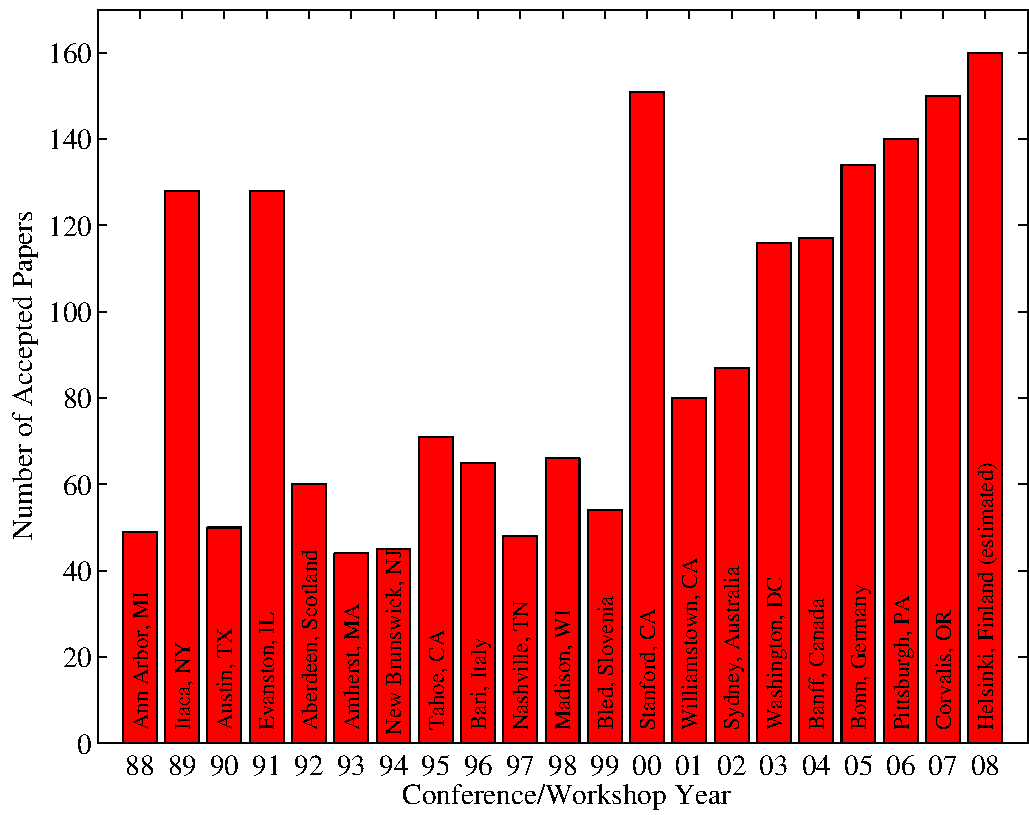
\includegraphics[width=\columnwidth]{icml_numpapers}}
%\caption{Historical locations and number of accepted papers for International
%Machine Learning Conferences (ICML 1993 -- ICML 2008) and International
%Workshops on Machine Learning (ML 1988 -- ML 1992). At the time this figure was
%produced, the number of accepted papers for ICML 2008 was unknown and instead
%estimated.}
%\label{icml-historical}
%\end{center}
%\vskip -0.2in
%\end{figure}




%\begin{algorithm}[tb]
%   \caption{Bubble Sort}
%   \label{alg:example}
%\begin{algorithmic}
%   \STATE {\bfseries Input:} data $x_i$, size $m$
%   \REPEAT
%   \STATE Initialize $noChange = true$.
%   \FOR{$i=1$ {\bfseries to} $m-1$}
%   \IF{$x_i > x_{i+1}$}
%   \STATE Swap $x_i$ and $x_{i+1}$
%   \STATE $noChange = false$
%   \ENDIF
%   \ENDFOR
%   \UNTIL{$noChange$ is $true$}
%\end{algorithmic}
%\end{algorithm}

%\subsection{Tables}
%
%
%% Note use of \abovespace and \belowspace to get reasonable spacing
%% above and below tabular lines.
%
%\begin{table}[t]
%\caption{Classification accuracies for naive Bayes and flexible
%Bayes on various data sets.}
%\label{sample-table}
%\vskip 0.15in
%\begin{center}
%\begin{small}
%\begin{sc}
%\begin{tabular}{lcccr}
%\toprule
%Data set & Naive & Flexible & Better? \\
%\midrule
%Breast    & 95.9$\pm$ 0.2& 96.7$\pm$ 0.2& $\surd$ \\
%Cleveland & 83.3$\pm$ 0.6& 80.0$\pm$ 0.6& $\times$\\
%Glass2    & 61.9$\pm$ 1.4& 83.8$\pm$ 0.7& $\surd$ \\
%Credit    & 74.8$\pm$ 0.5& 78.3$\pm$ 0.6&         \\
%Horse     & 73.3$\pm$ 0.9& 69.7$\pm$ 1.0& $\times$\\
%Meta      & 67.1$\pm$ 0.6& 76.5$\pm$ 0.5& $\surd$ \\
%Pima      & 75.1$\pm$ 0.6& 73.9$\pm$ 0.5&         \\
%Vehicle   & 44.9$\pm$ 0.6& 61.5$\pm$ 0.4& $\surd$ \\
%\bottomrule
%\end{tabular}
%\end{sc}
%\end{small}
%\end{center}
%\vskip -0.1in
%\end{table}
\section{Discussion and Outlook}

We have seen different methods for processing graphs on multiple scales, most of which depend on some form of convolutions on graphs. One category are spectral methods like wavelets and graph scattering transforms where only some rely on training weights. These methods usually require access to the full adjacency matrix and perform convolutions in the frequency domain. The other category are the mostly trainable methods, which rely on convolution in the vertex domain via some form of message passing using GNNs. This includes graph coarsening like GraphZoom, hierarchical clustering with DiffPool or scalable GNN architectures. While the latter perform better in many cases, the spectral methods may not be disregarded \cite{xu2018powerful},  when only little or perturbed training data is available, as can be seen in the case of the very flexible graph scattering transforms. With GWNN \cite{xu2019graph}, GDC \cite{klicpera2019diffusion} or the coarsening step in GraphZoom \cite{deng2020graphzoom}, we also saw that many modern approaches combine classical, spectral methods with modern GNN approaches to achieve new state of the art results.




%One disadvantage of spectral methods is that they usually require the full adjacency matrix of a graph (exception local...). 

In the future, we can expect more advances in the field of multi-scale learning on graphs through these combinations of deep learning methods with mathematically well founded spectral approaches like the graph wavelet transform. This allows to combine the advantages of spatial and spectral convolutions.


%Spectral (possibly global) vs. local convolutions, efficiency, performance, more common
%... works better than ...

%classic Spectral methods, while older and (at times not learnable) show to still be useful on themselves as well as helpers for modern architectures like in GraphZoom

%graph scattering transforms, while they can't learn perform well on ... and are flexible...









%TODO: Update citations (remove arXiv preprints where possible)

% In the unusual situation where you want a paper to appear in the
% references without citing it in the main text, use \nocite
%\nocite{langley00}


\bibliography{example_paper}
\bibliographystyle{icml2020}


%%%%%%%%%%%%%%%%%%%%%%%%%%%%%%%%%%%%%%%%%%%%%%%%%%%%%%%%%%%%%%%%%%%%%%%%%%%%%%%
%%%%%%%%%%%%%%%%%%%%%%%%%%%%%%%%%%%%%%%%%%%%%%%%%%%%%%%%%%%%%%%%%%%%%%%%%%%%%%%
% DELETE THIS PART. DO NOT PLACE CONTENT AFTER THE REFERENCES!
%%%%%%%%%%%%%%%%%%%%%%%%%%%%%%%%%%%%%%%%%%%%%%%%%%%%%%%%%%%%%%%%%%%%%%%%%%%%%%%
%%%%%%%%%%%%%%%%%%%%%%%%%%%%%%%%%%%%%%%%%%%%%%%%%%%%%%%%%%%%%%%%%%%%%%%%%%%%%%%
\appendix
\section{Appendix}
\subsection{Additional Figures}

\begin{figure}[ht]
	\vskip 0.2in
	\begin{center}
		\centerline{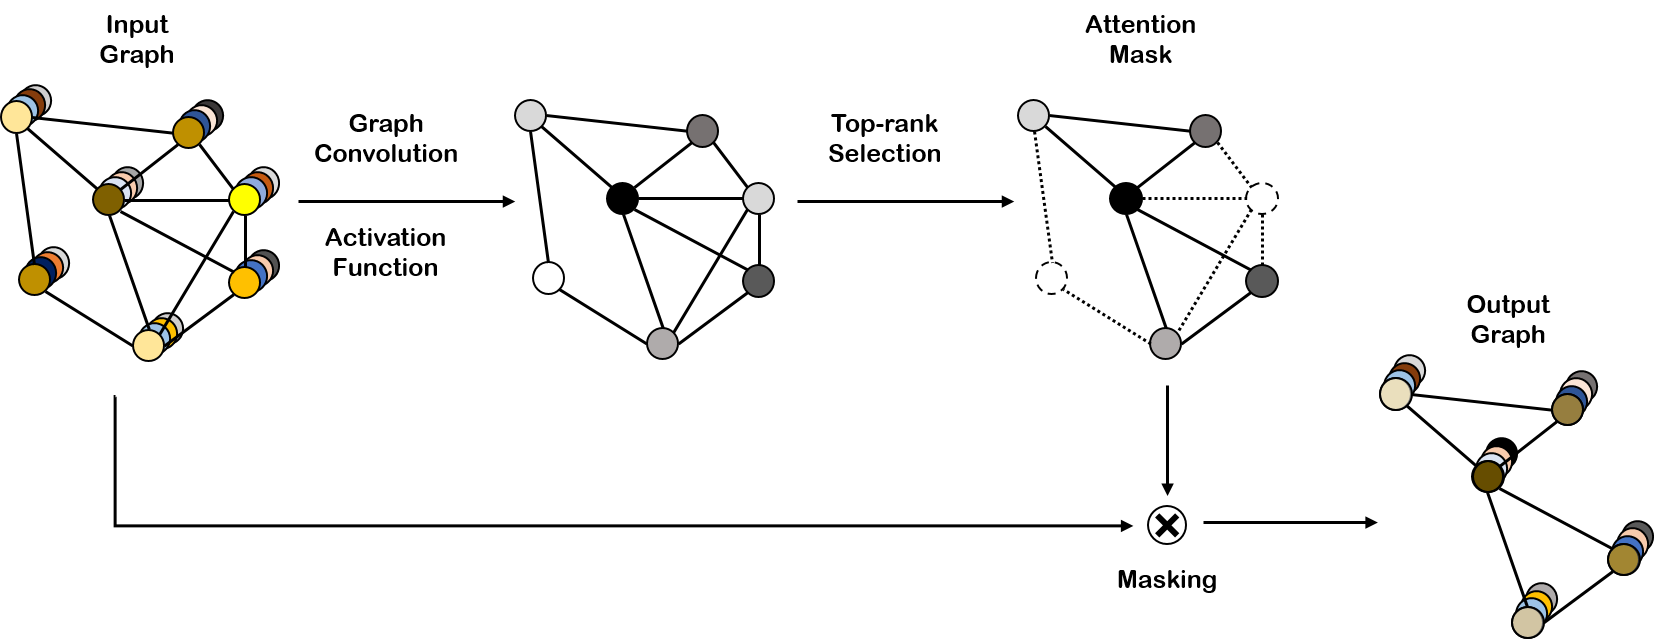
\includegraphics[width=\columnwidth]{sagpool}}
		\caption{The SAGpool attention mask decides which nodes are kept for the next layer. Figure from \cite{lee2019self}.}
		\label{fig:sagpool}
	\end{center}
	\vskip -0.2in
\end{figure}

\begin{figure}[ht]
	\vskip 0.2in
	\begin{center}
		\centerline{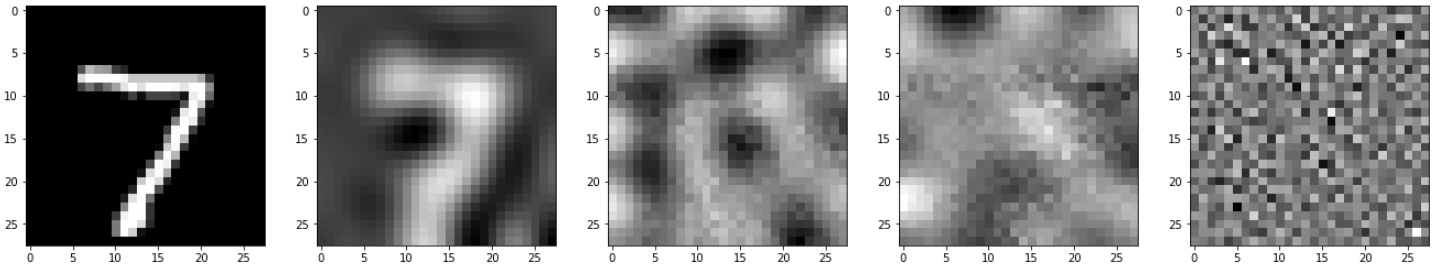
\includegraphics[width=\columnwidth]{scatteringresult}}
		\caption{Graph Scattering Transform on a grid graph of pixels. (left to right) input image, then: Graph Scattering Transform layers. Figure from \cite{zou2019graph}.}
		\label{fig:scatteringresult}
	\end{center}
	\vskip -0.2in
\end{figure}
\subsection{Convolution theorem}
\label{sec:convtheorem}
The convolution theorem\footnote{\href{https://en.wikipedia.org/wiki/Convolution_theorem}{https://en.wikipedia.org/wiki/Convolution\_theorem}} states that convolving the kernel $g$ over a signal $f$ is equivalent to first transforming $g$ and $f$ to frequency domain using $\mathcal{F}$, usually using a Fourier transformation, to achieve $\hat{g}=\mathcal{F}(g)$ and $\hat{f}=\mathcal{F}(f)$. Then the convolution in the spatial domain is equivalent to a multiplication in the frequency domain: \\ $f * g = \mathcal{F}^{-1}(\mathcal{F}(f)\cdot \mathcal{F}(g))$ %(todo: figure?,
%\subsection{Fourier transformation}
%\label{sec:fourier}
%Fourier transformation on euclidean data, mention sin/cosine


\subsection{Other methods}
\label{sec:other}
RecurrentGNNs \cite{ruiz2020gated} can be used for graphs modeling dynamic processes (like the initially mentioned spread of a novel disease) and therefore enable scaling in the time domain.

With scale as the size of the graph, the approaches vary with the number of nodes: For small graphs, different architectures are possible than for large graphs \cite{simonovsky2018graphvae,hamilton2017inductive}.
Learning on small graphs (like molecules) also allows for much more complex GNN architectures which are tuned for that task \cite{klicpera2020directional} in contrast to the simple architectures like SAGEConv or the model of \citet{wu2019simplifying} employed for larger graphs.



%%%%%%%%%%%%%%%%%%%%%%%%%%%%%%%%%%%%%%%%%%%%%%%%%%%%%%%%%%%%%%%%%%%%%%%%%%%%%%%
%%%%%%%%%%%%%%%%%%%%%%%%%%%%%%%%%%%%%%%%%%%%%%%%%%%%%%%%%%%%%%%%%%%%%%%%%%%%%%%


\end{document}


% This document was modified from the file originally made available by
% Pat Langley and Andrea Danyluk for ICML-2K. This version was created
% by Iain Murray in 2018, and modified by Alexandre Bouchard in
% 2019 and 2020. Previous contributors include Dan Roy, Lise Getoor and Tobias
% Scheffer, which was slightly modified from the 2010 version by
% Thorsten Joachims & Johannes Fuernkranz, slightly modified from the
% 2009 version by Kiri Wagstaff and Sam Roweis's 2008 version, which is
% slightly modified from Prasad Tadepalli's 2007 version which is a
% lightly changed version of the previous year's version by Andrew
% Moore, which was in turn edited from those of Kristian Kersting and
% Codrina Lauth. Alex Smola contributed to the algorithmic style files.
